\documentclass[11pt, conference]{IEEEtran}
\usepackage[spanish]{babel}
\usepackage[utf8]{inputenc}
\usepackage{amsmath}
\usepackage{amsfonts}
\usepackage{cite}
\usepackage{graphicx}

\begin{document}
\title{\bf Matrices y Determinantes}
\author{Diego David Alvarez Flores \\
Kevin Jhomar Sanchez Sanchez \\}
\maketitle

\pagebreak 

\tableofcontents 

\pagebreak
\section{Matrices}
Antes de iniciar poder encontrar mucha mas informacion especificada en y en 

\
\

\textbf{Definicion de Matrices}

\

En esta seccion nosotros vamos a comenzar nuestro estudio de la teoria de matrices dando algunas definiciones fundamentales del asunto. Nosotros vamos a ver como las matrices pueden ser combinadas a traces de las operaciones aritmeticas de adicion, sustraccion y multiplicacion, para luego establecer aplicaciones de la misma.

\

\begin{figure}[h]
	\begin{center}
		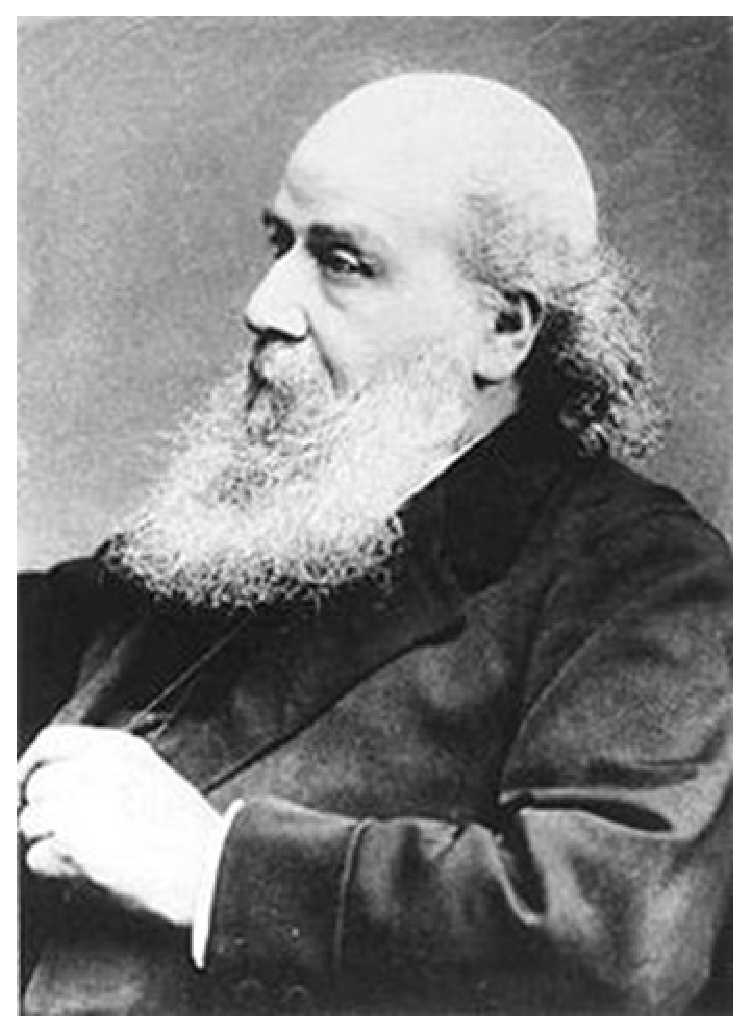
\includegraphics[scale=0.15]{img27.eps}
        \caption{Creador de la palabra Matriz\cite{Alfonso2010c}} 
	\end{center}
\end{figure}
\

Denominamos matriz a una tabla de elementos dispuestos en lineas y columnas. Por ejemplo, recogemos datos referentes a altura, peso y edad de un grupo de cinco personas en la siguiente tabla:

\begin{table}[htb]
\begin{center}
\begin{tabular}{|l|l|l|l|}
\hline
 & {\bf Altura}(metros) & {\bf peso}(kilogramos) & {\bf Edad }(años)  \\
\hline \hline
{\bf Persona 1} & 1,70 & 72 & 22 \\ \hline
{\bf Persona 2} & 1,65 & 68 & 24 \\ \hline
{\bf Persona 2} & 1,68 & 65 & 24 \\ \hline
{\bf Persona 4} & 1,75 & 80 & 33 \\ \hline
\end{tabular}
\end{center}
\end{table}

Si nosotros suprimimos los titulos, obtenemos la siguiente coleccion rectangular de numeros reales con cuatro filas y tres columnas, denomina {\textit{matriz}.

\

Una gran cantidad de otros conjuntos de datos tabulados forman naturalmente arreglos rectangulares. Veremos despues que un buen numero de calculos que deseamos realizasr con tales datos corresponden a ciertas operaciones con matrices que se definen posteriormente. 

\

{\bf Definicion.} Una {\textit{matriz}} es un agrupamiento  o arreglo rectangular de numeros ordenados en filas o columnas de la siguiente forma:
\[ A = \left[
\begin{array}{c c c c} 
a_{11} &a_{12}&\cdots &a_ {1n} \\
a_{22} &a_{23}&\cdots & a_{2n} \\
\vdots&\vdots&\ddots & \vdots \\
a_ {m1} & a_ {m2} &\cdots& a_{nn}
\end{array} \right] _ {mxn} \]

Donde los numeros {\textit {a ij} } son denomminados elementos o entradas de la matriz A.

\  

El {\textit{ orden}} o {\textit{dimension}} de la matriz 
esta dado por el producto indicado por {\textit{"m x n"}}, donde {\textit{m}} indica el numero de filas y {\textit{n}} indica el numero de columnas.

\

{\bf Notacion:} Las matrices se denotan por letras mayusculas y en forma abreviada y se escribe como $ A = (a_{ij})_ {mxn} $  . La matriz puede ser denotada por $ A=(a_{ij} )$ cuando se sobreentiende so orden o dimension.

\ 

El {\textit{conjunto de todas las matrices de orden  m x n}} es denotado por:
\[ M=
\left\{ \begin{array}{c}
A/A=(a_{ij}); i=1,2, ... ,m; j=1,2, ...,n
\end{array} \right\}  \]

{\bf Observaciones:}

\

\begin{enumerate} 
\item
Las matrices pueden asumir diferentes nombres, por ejemplo: {\textit{bloque rectangular, tabla de m filas y n columnas, etc.}} La forma como llamaremos a ese objeto matematico no es tan importante, pero si es la utilidad que demos a sus diferentes aplicaciones.

\item
el conjunto de elementos o componentes de una matriz no solo se encierra entre corchetes, sino tambien entre parentesis.
\end{enumerate} 

\

{\bf Ejemplos:}
\begin{enumerate} 
\item
$ A=\left[
\begin{array}{c c c c} 
-2&3&4&-2 \\
1&0&2&-3 \\
4&6&-7&10
\end{array} \right]_{3x4} $

\

, la matriz A es de orden 3 x 4, pues la matriz tiene 3 filas y 4 columnas.
\item
$ B=\left[
\begin{array}{c c c c c c} 
3&1&0&0&0&2\\
2&1&1&0&1&0\\
0&0&0&0&0&0\\
1&2&1&2&1&2
\end{array} \right]_{4x6} $ , la matriz B es de orden 4 x 6, pues la matriz consta de 4 filas y 6 columnas.
\item
$ C=\left[
\begin{array}{c} 
{x^2 }-1 \\
6\\
{x^3}-6x \\
x-1\\
2
\end{array} \right]_{5x1} $ 

\

, la matriz C es de orden 5 x 1(matriz columna).

\

\item 
$ D= \left[
\begin{array}{c c c c c} 
1&3&5&\cdots &97\\
4&1&1&\cdots &1\\
7&1&1&\cdots &1\\
\vdots&\vdots&\vdots&\ddots & \vdots \\
31&1&1&\cdots& 1

\end{array} \right]  $ 

\

, determine el orden de la matriz D.

\

{\bf \underline {Solucion:}}

\

Para determinar el numero de columnas de la matriz D, tomemos los elementos de la primera fila 1, 3, 5, ... , 97, donde se observaque estos son numeros impares consecutivos.

En consecuencia existe 49 numeros. Por tanto la matriz tiene 49 columnas.

\

En forma analoga, para determinar el numero de filas de la matriz D tomemos los elemntos de la primera columna 1, 4, 7 , ... ,31, donde estos numeros forman una progresion aritmetica. Entonces se tiene la siguiente formula $ a_n = a_1+(n-1)r $, donde $ a_n $ = 31(ultimo elemento) y la razon es r = 3. Entonces:
\begin{eqnarray}
  a_n = a_1+(n+1)r \nonumber \\
(n-1)r = a_n - a_1 \nonumber \\
n = {\frac{a_n - a_1}{r}} +1 \nonumber \\
n = {\frac{30}{3}} + 1 \nonumber\\
n = 11 \nonumber \\
\end{eqnarray}

Por lo tanto la matriz es de 11 filas.

Finalmente la matriz D es de orden 11 x 49

\item
Dada la matriz 

\

$ A = \left[\begin{array}{c c c c c c c c} 3&4&-1&4&5&-8&3&1\\4&5&-2&3&1&3&9&1\\6&1&5&7&1&1&0&0\\2&0&1&3&1&7&8&1 \end{array} \right]$ 

\

determine:

\

\begin{enumerate}
\item ${\frac{a_{23} + a_{45} }{a_{21} }} - 5_{ a_{27}}$
\item $ \sqrt{a_{34}+3_{a_{46}a_{33} }-12 } $
\end{enumerate}

\

{\bf \underline{Solucion:} }

\

\begin{enumerate}
\item ${\frac{a_{23} + a_{45} }{a_{21} }} - 5_{ a_{27}} = {\frac{-2+1}{4}}-5(9)=-{\frac{1}{4}}-45=-{\frac{181}{4}} $
\item $ \sqrt{a_{34}+3_{a_{46}a_{33} }-12 } =\sqrt{7+3(7)(5)-12} =10 $
\end{enumerate}
\item
Dado $B=(b_{ij})_{4x3} $

\

donde $b_{ij}= \left\{ \begin{array}{lll}
2_{j-i} &;& \mbox{Si $i < j$}\\
j &;& \mbox{Si $i = j$}\\
j-i&;& \mbox{Si $j>i$} \end{array} \right. $ 

\

, construya la matriz B.

\

{\bf \underline{Solucion:}}

\

$ B = \left[\begin{array}{c c c c} b_{11}&b_{12}&b_{13}\\b_{21}&b_{22}&b_{23}\\b_{31}&b_{32}&b_{33}\\b_{41}&b_{42}&b_{43}& \end{array} \right]$ = $ \left[\begin{array}{c c c} 1&3&5\\-1&2&4\\-2&-1&3\\-3&-2&-1 \end{array} \right]$

\

\ 

{\bf  Igualdad de matrices}

\

{\bf Definicion.} Sean las matrices $ A= (a_{ij})_{mxn}$ y $ B=(b_{ij})_{mxn}$.Se dice que las matrices $A$ y $B$ son igualessi, y solo si, son del mismo orden y sus respectivos elementos son iguales. Es decir:

\[ A=B   \Leftrightarrow  a_{ij} = b_{ij};\forall i,j\]

{\bf Ejemplo.} Determine $(2x + 3y - 5z)^2$, sabiendo que las matrices $A$y$B$ son iguales, donde:

\

$ A = \left[\begin{array}{c c c c} 1+x&2&y-x&9\\0&x+1&0&7\\z-1&-4&4&w \end{array} \right]$ y 

\

$B= \left[\begin{array}{c c c c} x+1&2&z&w\\0&3x-5&0&7\\x&-4&4&9 \end{array} \right] $

\

{\bf \underline{Solucion:}}

\

Por el dato del problema:
\[ 
{\left[\begin{array}{c c c c} 1+x&2&y-x&9\\0&x+1&0&7\\z-1&-4&4&w \end{array} \right]}  = {\left[\begin{array}{c c c c} x+1&2&z&w\\0&3x-5&0&7\\x&-4&4&9 \end{array} \right]}
\]

\

Luego por definicion de igualdad de matrices se tiene:

\

$\left\{ \begin{array}{llll}
y-x=z \\
x+1=3x-5 \forall x=3\\
z-1=x\\
w=9
\end{array} \right. $

\

reemplazando este valor obtenido en la tercera ecuacion , se obtiene {\textit{z}}=4. Luego, estos resultados los reemplazamos en la primera ecuacion y se obtiene {\textit{y}}=7.

\

Finalmente:$ (2x+3y-5z)^2=(2(3)+3(7)-5(4))^2 =49$


\end{enumerate}

\section{Tipos de Matrices}
\subsection{Matriz cuadrada}
Se dice de una matriz A es cuadrada cuando el número de filas coincide con el número de columnas.Es decir tiene la forma:
\[
  A = \left[
  \begin{array}{cccc}
  a_{11} &a_{12} & \cdots & a_{1n} \\
  a_{21} &a_{22} & \cdots & a_{2n} \\
  \vdots & \vdots &\ddots & \vdots \\
  a_{n1} &a_{n2} & \cdots & a_{nn} \\
  \end{array} \right]
  \medskip
\]

\

Se denomina elementos de la diagonal principal a los elementos $a_{11},\ a_{22}, \cdots,\ a_{nn}$

\

\smallskip
\textbf{Ejemplo:} \textnormal{Son matrices cuadradas las siguientes matrices:}
\[
	A = \left(
    \begin{array}{ccc}
    2 & 3 & 5 \\
    4 & 0 & 11 \\
    3 & 1 & 0 \\
    \end{array}
    \right),\quad 
    B = \left(
    \begin{array}{cccc}
    0 & 1 & 1 & 3 \\
    0 & 3 & 4 & 1 \\
    0 & 4 & 6 & 7 \\
    0 & 0 & 0 & 0 \\
    \end{array}
    \right),\quad etc.
\]
Mientras que no son Matrices cuadradas las siguientes matrices:
\[
	C = \left(
    \begin{array}{cccc}
    	2 & 3 & 0 & 1 \\
        4 & 2 & 0 & -3
    \end{array}
    \right),\quad
    D = \left[
    \begin{array}{ccccc}
		2 & 3 & -3 & 6 & 7 \\
        1 & 0 & 1 & 4 & 2 \\
        5 & 0 & -3 & 7 & -4 \\
	\end{array}	
    \right]\]
, etc.,pero si son matrices rectangulares

\

\subsection{Matriz columna}
Se llama matriz columna de orden $m \textnormal{x} 1$

\

\textbf{Ejemplo.} Son matrices columna:

\

\[
	A = \left[
	\begin{array}{c}
    	4\\
        3\\
        0\\
    \end{array}
    \right];\quad
    B = \left[
	\begin{array}{c}
    	0\\
        0\\
        0\\
        0\\
    \end{array}
	\right],\quad etc.
\]
\subsection{Matriz Fila}
Se llama matriz $fila$ a toda matriz de orden $1 \textnormal{x} n$
\[
	A = \left[
	\begin{array}{cccc}
    	1 & 0 & -1 & 0
    \end{array}
    \right]_{1x4};\quad
    B = \left[
	\begin{array}{cccccc}
    	2 & 2 & 3 & 1 & 3 & -5
    \end{array}
	\right]_{1x6},\quad etc.
\]
\subsection{Matriz Nula}
Se dice que una matriz es $nula$ cuando todos sus elementos son ceros y se denota por $\theta$
\[
	\theta = \left[
  \begin{array}{cccc}
  0 & 0 & \cdots & 0 \\
  0 & 0 & \cdots & 0 \\
  \vdots & \vdots &\ddots & \vdots \\
  0 & 0 & \cdots & 0 \\
  \end{array} \right]_{m\ \textnormal{x}\ n}
\]
\subsection{Matriz Diagonal}
Es aquella Matriz cuadrada cuyos elementos fuera fuera de la diagonal principal son ceros. Es decir:
\[
	D = \left(a_{ij}\right)_{n\ \textnormal{x}\ n} es\ una\ matriz\ diagonal \Longleftrightarrow a_{ij} = 0;\forall i \not = j.
\]
\[
	\theta = \left[
  \begin{array}{cccc}
  a_{11} & 0 & \cdots & 0 \\
  0 & a_{22} & \cdots & 0 \\
  \vdots & \vdots &\ddots & \vdots \\
  0 & 0 & \cdots & a_{nn} \\
  \end{array} \right]_{n\ \textnormal{x}\ n}
\]

\

\textbf{Ejemplo.}

\

$
	A = \left(
    \begin{array}{ccc}
    	1 & 0 & 0 \\
        0 & 6 & 0 \\
        0 & 0 & 9 \\
    \end{array}
    \right);\qquad
$    

\

\
    
$    
    B = \left[
    \begin{array}{cccc}
    	-2 & 0 & 0 & 0 \\
        0 & 6 & 0 & 0\\
        0 & 0 & 0 & 0 \\
        0 & 0 & 0 & 0 \\
    \end{array}
    \right]
    Son\ matrices\ diagonales.
$

\

\subsection{Matriz Escalar}
Es una matriz diagonal en la que todos los elementos de la diagonal principal son iguales. Es decir:

\

$
	E = \left(a_{ij}\right)_{n\ \textnormal{x}\ n} es una matriz escalar \Longleftrightarrow
    a_{ij} = 
    \left\{
    	\begin{array}{lc}
        	0 & ;\ si\ i \not = j \\
            k & ;\ si\ i = j \\
        \end{array}
    \right\}
$

\

\[
	E = \left[
  \begin{array}{cccc}
  k & 0 & \cdots & 0 \\
  0 & k & \cdots & 0 \\
  \vdots & \vdots &\ddots & \vdots \\
  0 & 0 & \cdots & k \\
  \end{array} \right]_{n\ \textnormal{x}\ n}
\]

\

\textbf{Ejemplo.}

\

$
	A = \left(
    \begin{array}{ccc}
    	6 & 0 & 0 \\
        0 & 6 & 0 \\
        0 & 0 & 6 \\
    \end{array}
    \right);\qquad
$

\

\

$
    B = \left[
    \begin{array}{cccc}
    	-2 & 0 & 0 & 0 \\
        0 & -2 & 0 & 0\\
        0 & 0 & -2 & 0 \\
        0 & 0 & 0 & -2 \\
    \end{array}
    \right]
    son\ matrices\ escalares.
$
\smallskip

\

$Observacion.$ Una matriz nula es una matriz escalar y a su vez es una matriz diagonal
\subsection{Matriz Identidad}
Es una matriz escalar en al que $k = 1$,Denotada por $I$. Es decir es de la forma:

\

\[
	I = \left[
  \begin{array}{cccc}
  1 & 0 & \cdots & 0 \\
  0 & 1 & \cdots & 0 \\
  \vdots & \vdots &\ddots & \vdots \\
  0 & 0 & \cdots & 1 \\
  \end{array} \right]_{n\ \textnormal{x}\ n}
\]
\textbf{Ejemplo.}
$
	I = \left[
    \begin{array}{cccc}
    	1 & 0 & 0 & 0 \\
        0 & 1 & 0 & 0\\
        0 & 0 & 1 & 0 \\
        0 & 0 & 0 & 1 \\
    \end{array}
    \right]
    es\ una\ identidad\ de\ ordern\ 4.
$
\subsection{Matriz Escalonada}
La matriz $A = \left(a_{ij}\right)_{m\ \textnormal{x}\ n}$ es escalonada si tiene la siguiente estructura:
	\begin{enumerate}
    	\item Las primeras $k$ filas son no nulas y las restantes $\left(m - k\right)$ son nulas.
        \item El primer elemento no nulo de cada una de las $k$ filas es la unidad.
        \item En cada una de las $k$ filas el numero de ceros anteriores al 1, crece de fila a fila 
    \end{enumerate}
\textbf{Ejemplo.} Las siguientes matrices son escalonadas:
\[
	A = \left[
    \begin{array}{cccc}
    1 & 7 & 0 & 0 \\
    0 & 1 & 3 & 4 \\
    0 & 0 & 0 & 0\\
    \end{array}
    \right],\quad 
    B = \left[
    \begin{array}{cccccc}
    1 & 2 & 3 & 6 & 0 & 0 \\
    0 & 1 & 0 & 0 & 3 & 4 \\
    0 & 0 & 0 & 1 & 3 & 7\\
    0 & 0 & 0 & 0 & 1 & 5 \\
    \end{array}
    \right],\quad etc.
\]

\

mientras que las siguientes no son escalonadas:

\

\[
	C = \left[
    \begin{array}{cccccc}
    1 & 0 & 0 & 0 & 0 & 0 \\
    0 & 1 & 0 & 3 & 4 & 5 \\
    0 & 0 & 1 & 0 & 2 & 3\\
    0 & 0 & 1 & 3 & 4 & 4 \\
    \end{array}
    \right],\quad
    D = \left(
    \begin{array}{cccc}
    3 & 0 & 4 & 8 \\
    0 & 1 & 8 & 8 \\
    0 & 0 & 0 & 1\\
    0 & 0 & 1 & 5\\
    \end{array}
    \right),\quad etc.
\]

\

\section{Operaciones con matrices}
\subsection{Multiplicacion de una matriz por un escalar}
\smallskip
\textbf{Definicion.} Dada la matriz $A = \left(a_{ij}\right)_{m\ \textnormal{x}\ n}$ y dado un numero real para $\alpha$, el $producto\ de\ \alpha\ por A$ esta dado por:

\

\[
	\alpha\!A = \left[
  \begin{array}{cccc}
  \alpha\!a_{11} & \alpha\!a_{12} & \cdots & \alpha\!a_{1n} \\
  \alpha\!a_{21} & \alpha\!a_{22} & \cdots & \alpha\!a_{2n} \\
  \vdots & \vdots &\ddots & \vdots \\
  \alpha\!a_{m1} & \alpha\!a_{m2} & \cdots & \alpha\!a_{mn} \\
  \end{array} \right]_{m\ \textnormal{x}\ n}
\]

\

\begin{center}
	\textbf{Observación.} Dada la matriz $A = \left(a_{ij}\right)_{m\ \textnormal{x}\ n}$, en particular se tiene:$-A = \left(-1\right)A = \left(a_{ij}\right)_{m\ \textnormal{x}\ n}$
\end{center}
\textbf{Ejemplo.} Dado la matriz
$
	D = \left[
    \begin{array}{ccc}
    2 & 3 & 1 \\
    3 & -4 & 5 \\
    1 & 7 & 9\\
    \end{array}
    \right]
$, entonces:

\

\[
	3A = \left[
    \begin{array}{ccc}
    3(2) & 3(3) & 3(1) \\
    3(3) & 3(-4) & 3(5) \\
    3(1) & 3(7) & 3(9) \\
    \end{array}
    \right]
     = \left[
    \begin{array}{ccc}
    6 & 9 & 3 \\
    9 & -12 & 15 \\
    3 & 21 & 27 \\
    \end{array}
    \right],\quad etc.
\]
\subsection{Adicion de Matrices}

\

\textbf{Definicion.} Sean las Matrices $A = \left(a_{ij}\right)_{m\ \textnormal{x}\ n}$ y $B = \left(b_{ij}\right)_{m\ \textnormal{x}\ n}. A + B$ es llamada suma de $A\ y\ B$, cuyo elemento general  es $\left(a_{ij}\right)_{m\ \textnormal{x}\ n} + \left(b_{ij}\right)_{m\ \textnormal{x}\ n}$

\

\[
	A+B = \left[
  \begin{array}{cccc}
  a_{11}+b_{11} & a_{12}+b_{12} & \cdots & a_{1n}+b_{1n} \\
  a_{21}+b_{21} & a_{22}+b_{22} & \cdots & a_{2n}+b_{2n} \\
  \vdots & \vdots &\ddots & \vdots \\
  a_{m1}+b_{m1} & a_{m2}+b_{m2} & \cdots & a_{mn}+b_{mn} \\
  \end{array} \right]_{m\ \textnormal{x}\ n}
\]

\

\begin{center}
	\textbf{Observación.} Para que exista la suma de dos matrices, éstas tienen que ser  del mismo order. Caso contrario no está definida.
\end{center}

\

\textbf{Propiedades:} Sean Matrices $A,B y c$ mientras del conjunto $
M^{m\textnormal{x}n}$(conjunto de matrices de orden m x n). Entonces:

\

\begin{enumerate}
	\item Conmutatividad: $A+B = B+A$
    \item Asociatividad: $(A+B)+C = A+(B+C)$
    \item Elemento Neutro: $\forall A \in M^{m\textnormal{x}n}, \exists\theta\in M^{m\textnormal{x}n}$ tal que  $A+(-A) = \theta$,donde $\theta$ es la matriz nula de orden $m\textnormal{x}n$
    \item Elemento inverso aditivo: $\forall A \in M^{m\textnormal{x}n}, \exists\theta(-A)\in M^{m\textnormal{x}n}$ tal que  $A+\theta = \theta$,donde $\theta$ es la matriz nula de orden $m\textnormal{x}n$
    \item Distributiva: 
    
    $\alpha(A+B) = \alpha\!A + \alpha\!B; \alpha \in \mathbb{R}$
       
    $A(\alpha+B) = \alpha\!A + \beta\!A; \alpha,\beta \in \mathbb{R}$
    \item Multiplicacion por 1: $1 \cdot A = A$ 
\end{enumerate}

\

El conjunto de matrices $M^{m\textnormal{x}n}$, cuyos elementos verifican las propiedades mencianadas, es llamado $\textbf{espacio vectorial de matrices}$

\

\subsection{Diferencia de Matrices}

\textbf{Definicion.} Dada las matrices del mismo orden $A$ y $B$. La diferencia de las matrices $A$ y $B$ se define como: $A-B=A(-1)B$

\

\textbf{Ejemplos.}
\begin{enumerate}
	\item Dada las matrices 
    $
      A = \left[
      \begin{array}{cccc}
      2 & 1 & 0 & 3 \\
      -1 & 0 & 2 & 3 \\
      1 & 4 & 2 & 7\\
      \end{array}
      \right]
    $ y $
      B = \left[
      \begin{array}{cccc}
      -4 & 3 & 2 & 0 \\
      1 & -2 & 4 & 5 \\
      2 & -2 & 1 & 0\\
      \end{array}
      \right]
    $
    
    \
    
    , determine las matrices A+B y A-B
    
    \
    
    {\bf \underline{Solucion:}}
    \[
    	A+B = \left[
        \begin{array}{cccc}
        2-4 & 1+3 & 0+2 & 3+0 \\
        -1+1 & 0-2 & 2+4 & 3+5 \\
        1+2 & 4-2 & 2+1 & 7+0\\
        \end{array}
        \right]
    \]
    \[
    	A+B = \left[
        \begin{array}{cccc}
        -2 & 4 & 2 & 3 \\
        0 & -2 & 6 & 8 \\
        3 & 2 & 3 & 7\\
        \end{array}
        \right]
    \]
    \[
    	A-B = \left[
        \begin{array}{cccc}
        2+4 & 1-3 & 0-2 & 3-0 \\
        -1-1 & 0+2 & 2-4 & 3-5 \\
        1-2 & 4+2 & 2-1 & 7-0\\
        \end{array}
        \right]
    \]
    \[
    	A-B= \left[
        \begin{array}{cccc}
        6 & -2 & -2 & 3 \\
        0 & 2 & -2 & -2 \\
        -1 & 6 & 1 & 7\\
        \end{array}
        \right]
    \]
    \item Dada las matrices
    
    \
    
    $
      A = \left[
      \begin{array}{ccc}
      \frac{1}{3} & 4 & \frac{2}{3} \\
      1 & 0 & 2 \\
      \frac{5}{3} & -2 & 1 \\
      \end{array}
      \right]
    $ y $
      B = \left[
      \begin{array}{ccc}
      1 & 2 & 4 \\
      \frac{1}{5} & -2 & \frac{3}{5} \\
      0 & 1 & -1 \\
      \end{array}
      \right]
    $
    
    \
    
    determine la matriz $M = 15(A+B-I)$, donde I es una matriz identidad ed orden 3
    
    \ 
	
    {\bf \underline{Solucion:}}
    
    \
    
    $M = 15A+15B-15I$
    
    $
      M = 15 \left[
      \begin{array}{ccc}
      \frac{1}{3} & 4 & \frac{2}{3} \\
      1 & 0 & 2 \\
      \frac{5}{3} & -2 & 1 \\
      \end{array}
      \right]
      + 15 \left[
      \begin{array}{ccc}
      1 & 2 & 4 \\
      \frac{1}{5} & -2 & \frac{3}{5} \\
      0 & 1 & -1 \\
      \end{array}
      \right]
      +15 \left[
      \begin{array}{ccc}
      1 & 0 & 0 \\
      0 & 1 & 0 \\
      0 & 0 & 1 \\
      \end{array}
      \right]
    $
    
    $
      M = \left[
      \begin{array}{ccc}
      5 & 60 & 10 \\
      15 & 0 & 30 \\
      25 & -30 & 15 \\
      \end{array}
      \right]
      + \left[
      \begin{array}{ccc}
      15 & 30 & 60 \\
      3 & -30 & 9 \\
      0 & 15 & -15 \\
      \end{array}
      \right]
      + \left[
      \begin{array}{ccc}
      15 & 0 & 0 \\
      0 & 15 & 0 \\
      0 & 0 & 15 \\
      \end{array}
      \right]
    $
    
    $
      M = \left[
      \begin{array}{ccc}
      5 & 90 & 70 \\
      18 & -45 & 39 \\
      25 & -15 & -15 \\
      \end{array}
      \right]
    $
\end{enumerate}
\subsection{Multiplicacion de matrices}
\textbf{Definicion.} Sean las Matrices $A = \left(a_{ij}\right)_{m\ \textnormal{x}\ p}$ y $B = \left(b_{ij}\right)_{p\ \textnormal{x}\ n}$ . El producto de $AB$ es una matriz de orden m x n cuyo termino general esta dado por:
\[
	c_{ij} = a_{i1} \cdot b_{1j} + a_{i2} \cdot b_{2j} + \cdots + a_{ip} \cdot b_{pj} = \sum_{k=1}^{p}a_{ik}\cdot b_{kj}
\]
\begin{center}
Es decir, $c_{ij}$ se obtiene multiplicando la $i$-ésima fila de $A$ por $j$-ésima columna de $B$.
\end{center}
\textbf{Propiedades:} Supongamos que los tamaños de las matrices son tales que las operaciones indicadas pueden ser efectuadas. Entonces:
\begin{enumerate}
	\item $A(BC) = (AB)C$
    \item $(A+B)C = AC+BC$
    \item $A(B+C) = AB+AC$
    \item $AB\not=BA$(el producto de matrices es no conmutativo)
    \item $AI_{n} = A$ y $I_{m}A = A$, donde $A = (a_{ij})_{m\ \textbf{x}\ n}; I_{n}$ es la matriz identidad de orden n y $I_{m}$ es la matriz indentidad de orden $n$
\end{enumerate}
\bigskip
\bigskip
\bigskip
\section{Determinantes}

Los determinantes fueron introducidos en occidente a partir del siglo XVI , esto es , antes que la matrices que no aparecieron hasta el siglo XIX. Algunos de los mas grandes dematematicos de los siglos SVIII y XIX contribuyeronn al desarrollo de las propiedades de los determinantes. La mayoria de los historiadores coinciden en afirmar que la teoria de los determinantes se origino con el matematico Aleman Goofred Wilhelm Leibniz (1646-1716) quien fue , con Newton , el co-inventor del calculo diferencial e integral . Leibniz empleo los determiantes en 1693 con relacion a los sistemas de ecuaciones lineales simultaneas . No obstante , hay quienees creen que el matematico Japones Seki Kowa hizo lo mismo unos diez años antes . Las contribuciones mas prolificas a la teoria de los determinantes fueron las del matematico frances Agustin-Louis Cauchy(1789-1857). Cauchy escribio en 1812, una memoria de 84 paginas que contenia la primera demostracion del teorema $det(AB)= det (A) det(B)$. 
\begin{figure}[h]
	\begin{center}
		
\includegraphics[scale=0.15]{img25.eps}
        \caption{Matematico Aleman Goofried Wilhelm Leibniz} 
	\end{center}
\end{figure}
\begin{figure}[h]
	\begin{center}
		
\includegraphics[scale=0.15]{img26.eps}
        \caption{Matematico Frances Agustin-Louis Cauchy(1789-1857)} 
	\end{center}
\end{figure}
\subsection{Definición de determinantes}
\medskip
\textbf{Definición} Sea $M_{ixj}$el conjunto de matrices de orden $nxn$ . El determinante viene a ser una funcion que hace corresponder a cada matriz cuadrada $A$ un numero real. Es decir:
\\
\[|.| : M_{n\ x\ n}\ \rightarrow \ \mathbb{R} \]
\[A\ \rightarrow \ |A|\]



\end{document}
